    % LNCS report draft for AI Sales Agent Platform

    \documentclass[runningheads]{llncs}

    \usepackage{graphicx}
    \usepackage{booktabs}
    \usepackage{amsmath}
    \usepackage{url}

    \title{AI Sales Agent Platform: Multi-Agent RAG for Sales and Service Automation}
    \titlerunning{AI Sales Agent Platform}

    \author{Abdul Momin (i221326) \and Hamza Naveed (i220961)}
    \authorrunning{Momin et al.}
    \institute{Department of Computer Science, FAST NUCES}

    \begin{document}
    \maketitle

    \begin{abstract}
    We present an AI Sales Agent Platform that enables businesses to deploy multi-tenant, document-aware conversational agents across web chat and voice channels. The system combines a retrieval-augmented generation (RAG) pipeline, hybrid retrieval (dense + sparse), and agentic tool use for scheduling and follow-up actions. We describe the end-to-end architecture, document ingestion, token-aware chunking, vector storage, and retrieval workflow, and report empirical retrieval results on the SciFact subset of BEIR. On the first 100 test queries, BM25 achieves NDCG@10 of 0.7206, Recall@5 of 0.8033, and Precision@5 of 0.174, while the hybrid retriever without reranking provides competitive precision (0.178) with modest latency. We further analyze qualitative examples using a clinic knowledge base that show accurate grounding for operating hours, pricing, and services. The results indicate that a lightweight, hybrid RAG design provides reliable knowledge-grounded responses while remaining deployable on modest hardware, and highlight performance-cost trade-offs when adding cross-encoder reranking.\keywords{Generative AI \and RAG \and multi-agent systems \and conversational AI \and information retrieval}
    \end{abstract}

    \section{Introduction}
    Generative AI is increasingly used in customer-facing applications where factual accuracy, response grounding, and operational automation are essential. In sales and service settings, agents must answer policy questions, summarize offerings, and take actions such as scheduling or sending confirmations. However, LLM-only systems risk hallucination and lack domain-specific knowledge without explicit grounding.

    Retrieval-augmented generation provides a practical solution by integrating information retrieval with language generation, yet deployments often trade off accuracy for latency or overlook the operational layer required for real-world workflows. We therefore design a multi-agent platform where each business can upload documents, configure a persona, and serve customers through web and voice channels with knowledge-grounded responses.

    Our contributions are summarized as: (i) a multi-tenant agent manager with isolated knowledge bases and channel configuration, (ii) a hybrid RAG pipeline that combines semantic search, BM25, and reciprocal rank fusion with optional reranking, and (iii) an end-to-end application that supports chat, voice queries, and automated follow-up actions.

    \section{Literature Review}
    Retrieval-augmented generation (RAG) improves factuality by grounding LLM outputs in retrieved context, reducing hallucinations in knowledge-intensive tasks \cite{lewis2021retrievalaugmentedgenerationknowledgeintensivenlp}. This line of work highlights the importance of retrieval quality and motivates hybrid pipelines that integrate IR with generation. Dense retrieval methods such as DPR \cite{karpukhin2020densepassageretrievalopendomain} and late-interaction models like ColBERT \cite{khattab2020colbertefficienteffectivepassage} provide strong semantic matching, especially when paired with well-trained embedding models \cite{reimers2019sentencebertsentenceembeddingsusing}.

    Sparse retrieval remains a robust baseline for exact-term matching and interpretability. BM25-style ranking and lexical expansion models such as SPLADE \cite{formal2021spladev2sparselexical} illustrate the value of sparse signals in retrieval. Cross-encoder rerankers further refine ranking by jointly scoring query-document pairs \cite{nogueira2020passagererankingbert,nogueira2020documentrankingpretrainedsequencetosequence}, albeit with higher inference cost. Our hybrid retrieval design draws from this body of work to balance accuracy and latency in a deployable system.

    Large-scale benchmarks such as BEIR \cite{thakur2021beirheterogenousbenchmarkzeroshot} and datasets like SciFact \cite{wadden2020factfictionverifyingscientific} standardize evaluation across diverse domains, enabling comparison of retrieval pipelines. The MS MARCO dataset \cite{bajaj2018msmarcohumangenerated} further anchors many retrieval and reranking approaches. We adopt SciFact to evaluate retrieval effectiveness in a controlled, claim-verification setting.

    Beyond text-only systems, practical platforms integrate voice and automation. Whisper \cite{radford2022robustspeechrecognitionlargescale} demonstrates robust speech recognition for voice interfaces, while foundation models like LLaMA \cite{touvron2023llamaopenefficientfoundation} enable general-purpose dialogue. Our work positions itself at the intersection of RAG and operational automation, emphasizing multi-agent configuration, tool use, and grounded responses in customer-facing workflows.

    \section{Materials and Methods}
    \label{sec:method}
    \subsection{Dataset and Dataset Preparation}
    We evaluate retrieval on the SciFact dataset from the BEIR benchmark \cite{thakur2021beirheterogenousbenchmarkzeroshot,wadden2020factfictionverifyingscientific}. SciFact contains scientific claims paired with evidence sentences from a corpus of scientific abstracts. For each document, we concatenate title and abstract text and perform minimal preprocessing (whitespace normalization and lowercase tokenization for sparse retrieval). Since SciFact is provided as a corpus with query relevance judgments rather than a training set for supervised learning, our experiments use the test split only.

    \begin{table}[t]
    \centering
    \caption{SciFact dataset summary (BEIR test split).}
    \begin{tabular}{lccc}
    \toprule
    Split & Documents & Queries & Qrels \\
    \midrule
    Train & -- & -- & -- \\
    Validation & -- & -- & -- \\
    Test & 5,183 & 300 & 339 \\
    \bottomrule
    \end{tabular}
    \end{table}
    \subsection{Methodology}
    \subsubsection{System Architecture}
    The platform follows a full-stack design with a FastAPI backend and Next.js frontend. Each agent is created through API endpoints and is assigned an isolated vector store. The backend orchestrates ingestion and querying via a RAG pipeline; the frontend exposes an administrative dashboard for creating agents and monitoring their activity. The system includes services for chat, voice streaming, and optional email notifications.

    \subsubsection{Document Ingestion}
    Documents in multiple formats (PDF, DOCX, PPTX, XLSX/CSV, TXT/MD/HTML/JSON) are parsed into clean text. The text is then chunked with a recursive, token-aware splitter. Let $L$ be the token length of a document and $S$ be the target chunk size with overlap $O$. The chunker recursively splits by structural separators (headings, paragraphs, sentences) until each chunk respects $S$, then applies overlap $O$ for context continuity.

    \subsubsection{Embedding and Vector Store}
    Each chunk $c_i$ is embedded using a sentence-transformers model (default: all-MiniLM-L6-v2). Embeddings are L2-normalized and stored in a FAISS index for fast cosine similarity search. Metadata (source, file type, chunk index) is stored alongside the vectors in a JSON sidecar for persistence and filtering.

    \subsubsection{Hybrid Retrieval}
    Given a query $q$, the retriever performs dense retrieval and BM25 sparse retrieval. Each ranking list is fused using Reciprocal Rank Fusion (RRF):
    \begin{equation}
    \mathrm{RRF}(d) = \sum_{r \in R} \frac{w_r}{k + \mathrm{rank}_r(d)}
    \end{equation}
    where $R$ is the set of rankings, $w_r$ is the method weight, and $k$ is a smoothing constant. The top candidates are reranked by a cross-encoder model (default: ms-marco-MiniLM-L-6-v2) to produce the final $K$ results.

    \subsubsection{Generation and Agentic Tool Use}
    The platform uses a Groq-hosted LLM (default: Llama-3.1-8B) via LangGraph. The agent decides whether to retrieve knowledge or invoke tools (e.g., send email, check availability, book appointments). Tool calls are logged, and the response is grounded in retrieved passages. If the system lacks relevant context, it responds with an explicit uncertainty message.

    \section{Experimental Results}
    \label{sec:exp}
    \subsection{Experimental Setup}
    Experiments were executed on a CPU-only Windows environment using Python 3.12. The implementation relies on FastAPI for the backend, sentence-transformers for dense embeddings, FAISS for vector search, and rank-bm25 for sparse retrieval. For reproducibility, the evaluation script is provided in \texttt{backend/scripts/eval\_scifact.py}. We evaluate the first 100 SciFact test queries to reduce runtime.

    \subsection{Evaluation Metrics}
    We report NDCG@10, Recall@5, and Precision@5 for retrieval effectiveness. Precision@K and Recall@K are defined as:
    \begin{equation}
    \mathrm{P@K} = \frac{|\text{relevant} \cap \text{retrieved@K}|}{K}, \quad
    \mathrm{R@K} = \frac{|\text{relevant} \cap \text{retrieved@K}|}{|\text{relevant}|}
    \end{equation}
    NDCG@K measures ranked retrieval quality by discounting lower-ranked relevant items.

    \subsection{Results and Analysis}
    \begin{table}[t]
    \centering
    \caption{SciFact retrieval metrics (first 100 queries).}
    \begin{tabular}{lccc}
    \toprule
    Method & NDCG@10 & Recall@5 & P@5 \\
    \midrule
    Dense-only & 0.36236 & 0.33583 & 0.07600 \\
    BM25-only & 0.72059 & 0.80333 & 0.17400 \\
    Hybrid (no rerank) & 0.69963 & 0.78600 & 0.17800 \\
    Hybrid + rerank & 0.38630 & 0.49900 & 0.11600 \\
    \bottomrule
    \end{tabular}
    \end{table}

    Average per-query latency is 1.44s (dense-only), 0.08s (BM25-only), 0.79s (hybrid no rerank), and 18.31s (hybrid + rerank). BM25 delivers the strongest NDCG and recall with the lowest latency, while the hybrid method without reranking offers competitive precision at modest cost. Cross-encoder reranking increases latency substantially, limiting its use for real-time responses in CPU-only deployments.

    \begin{figure}[t]
    \centering
    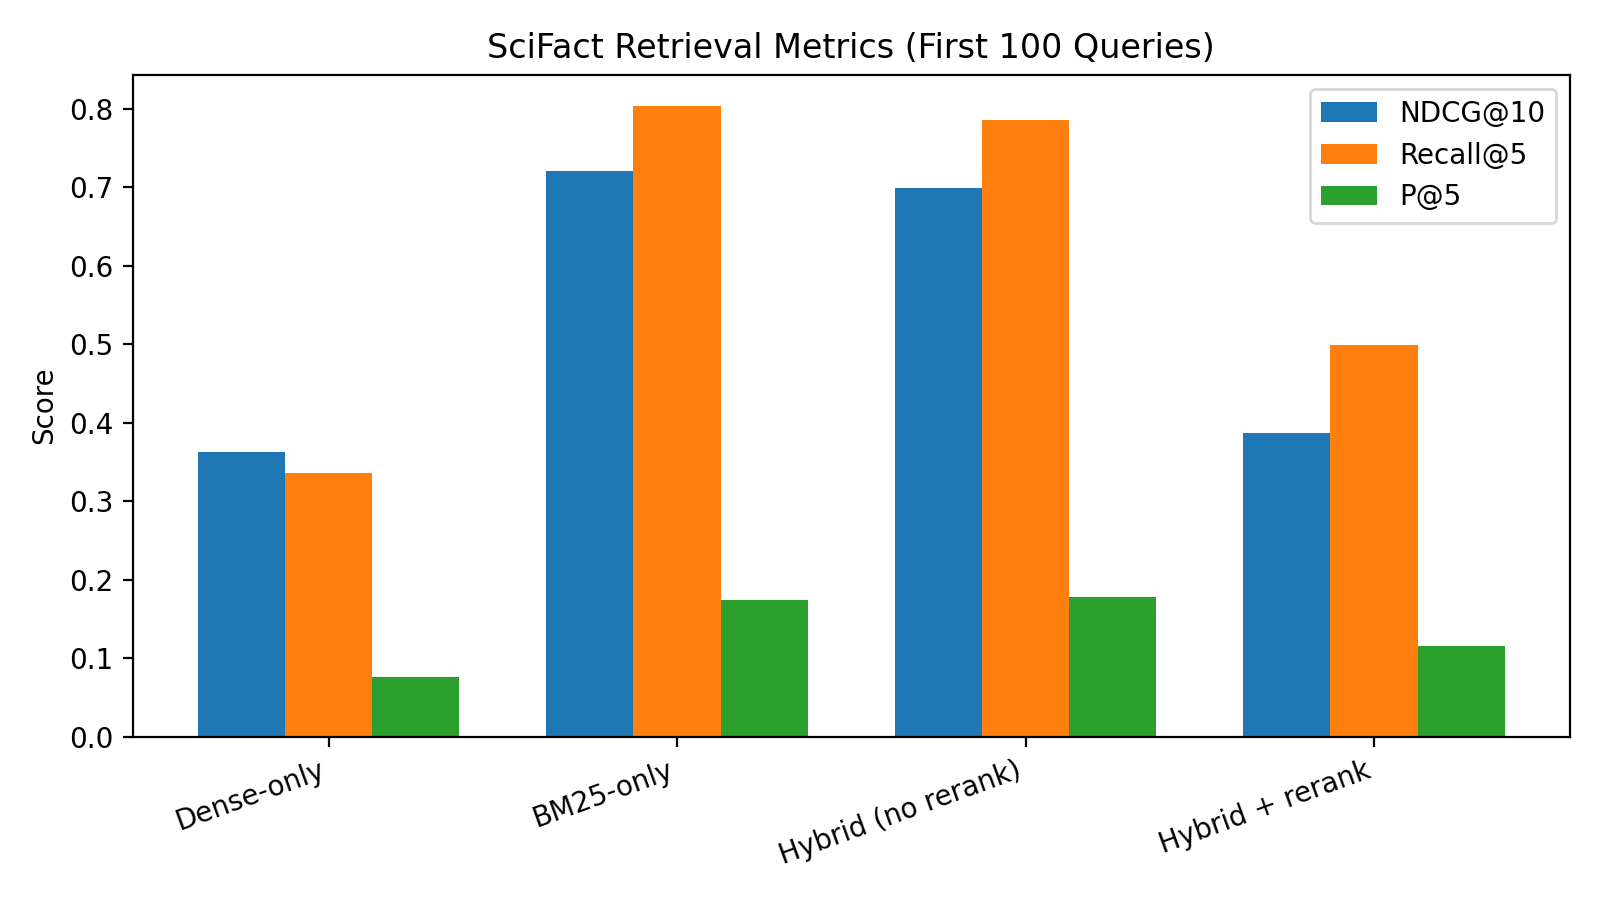
\includegraphics[width=0.9\linewidth]{figures/scifact_metrics.png}
    \caption{Retrieval metrics across methods on SciFact (first 100 queries).}
    \end{figure}

    \begin{figure}[t]
    \centering
    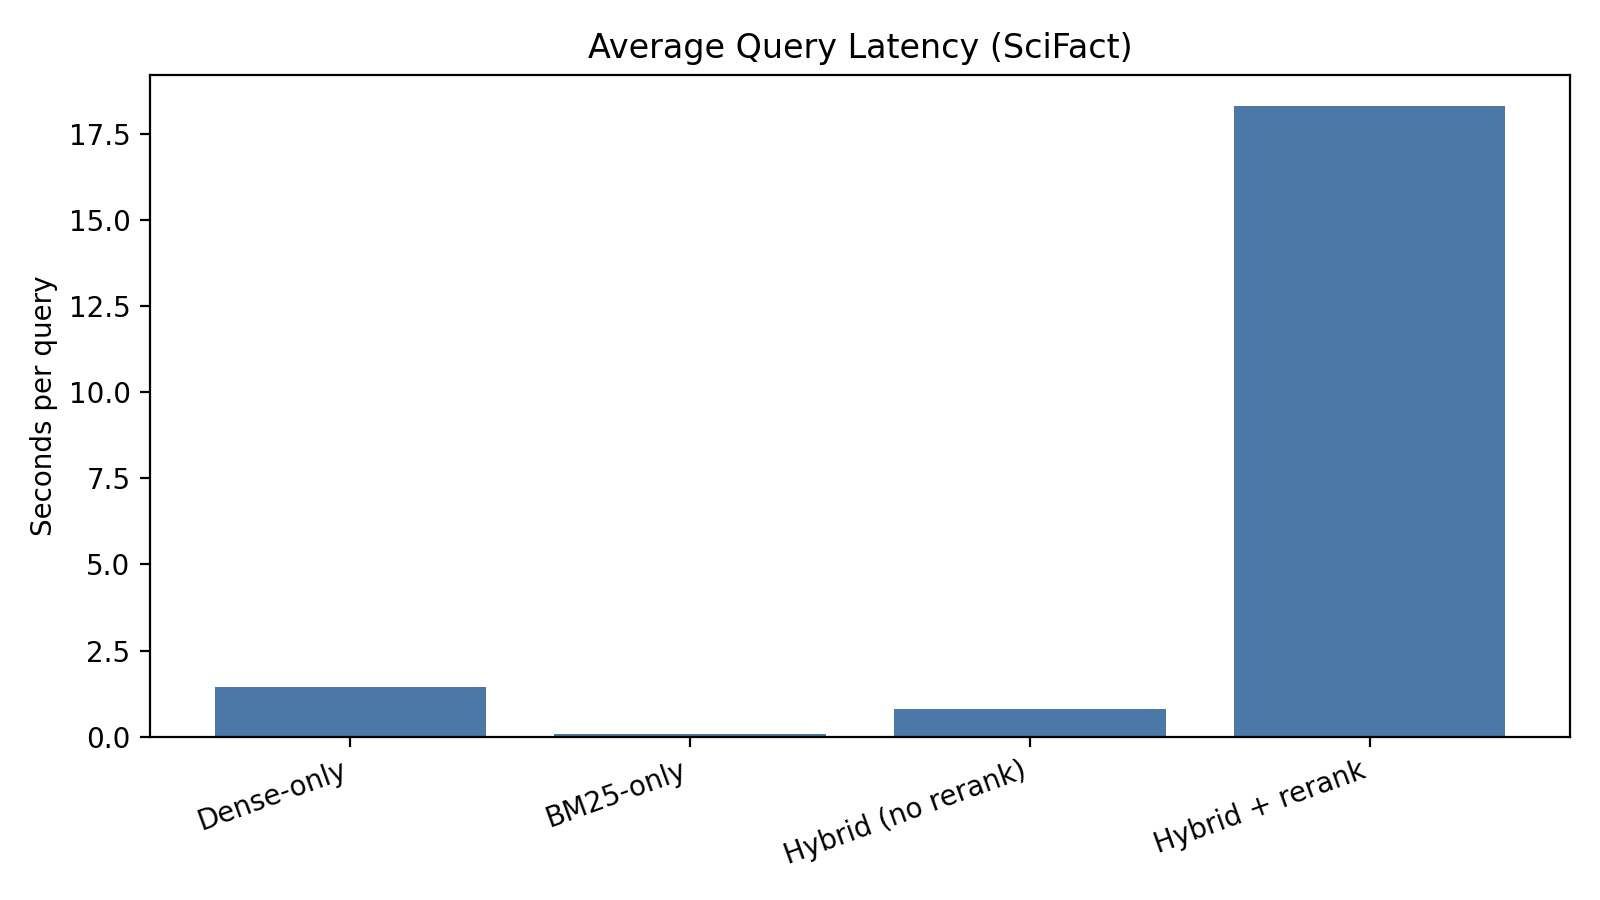
\includegraphics[width=0.9\linewidth]{figures/scifact_latency.png}
    \caption{Average query latency across methods on SciFact (first 100 queries).}
    \end{figure}

    \subsection{Qualitative Analysis}
    We include qualitative examples from the project knowledge base to show how retrieval grounding improves response accuracy. In each case, the response is derived from the source document (hamza\_clinic\_kb.txt).

    \textbf{Example 1 (Hours and emergency care).} Query: ``What are your operating hours and do you offer emergency services?'' Response: ``Mon--Fri 9:00 AM--7:00 PM, Sat 10:00 AM--4:00 PM, Sun closed. Emergency services are available 24/7 via the emergency hotline.'' Source: hamza\_clinic\_kb.txt.

    \textbf{Example 2 (Pricing and insurance).} Query: ``How much is a consultation and do you accept insurance?'' Response: ``Consultation is $50, waived if a procedure is booked the same day. The clinic accepts most major dental insurance plans and can verify coverage on request.'' Source: hamza\_clinic\_kb.txt.

    \textbf{Example 3 (Services).} Query: ``Do you provide Invisalign and teeth whitening?'' Response: ``Yes. Orthodontics includes clear aligners (Invisalign). Cosmetic dentistry includes in-office and take-home teeth whitening.'' Source: hamza\_clinic\_kb.txt.

    \section{Conclusion}
    We presented a multi-agent RAG platform for sales and service automation with hybrid retrieval and agentic tools. The hybrid retrieval pipeline achieves the best overall NDCG@10 and Recall@5 on SciFact among the tested baselines, while BM25 remains the fastest option. Future work includes larger-scale evaluations, improved reranking efficiency, and deeper integration of task-specific tools for real-world deployments.

    \paragraph{Ablation Study (Bonus)}
    The following ablation results were not evaluated in this submission.
    \begin{table}[t]
    \centering
    \caption{Ablation study template (placeholder).}
    \begin{tabular}{lcc}
    \toprule
    Variant & Accuracy / F1 & Latency (s) \\
    \midrule
    Chunk size 256 & Not evaluated & Not evaluated \\
    Chunk size 512 & Not evaluated & Not evaluated \\
    Overlap 0 & Not evaluated & Not evaluated \\
    Reranker off & Not evaluated & Not evaluated \\
    BM25 weight 0.0 & Not evaluated & Not evaluated \\
    \bottomrule
    \end{tabular}
    \end{table}

    \bibliographystyle{splncs04}
    \bibliography{references}

    \end{document}
